\section{評価及び考察}
本システムの識別精度と登録及び認証処理にかかる時間を確認するため,実験を行った.
まず,端末を持ち上げるモーションを対象とした識別精度の評価実験を行った.
本システムを用いてあらかじめ6名の被験者にモーションを4回入力してもらい,データの収集を行った.
各被験者ごとに,最初の3回分を登録モードにおける訓練データとして用い,最後の1回分を認証モードにおける入力データとして10回認証を試行した.
また,それぞれの試行時になりすまし認証データとして筆者自身が同様のモーションを入力して得たデータも入力した.
識別器より得られたデータを各被験者ごとに平均してまとめたものを表\ref{auth-result}に示す.

結果から,被験者Aと被験者B,被験者Fについては識別できているとわかる.
だが他の3名についてはなりすまし認証のデータで得られた識別器の出力がより低く出ており,識別できていない.
本システムでは,端末所有者のデータとなりすまし認証によるデータを識別するためにダミーデータを用いた.
ダミーデータは元データの値域及び次元数に依存するため,これらが小さい場合は元データとの差があまり出ない可能性がある.
これにより,端末所有者が入力したデータであってもなりすまし認証であると識別されてしまったのではないかと考えられる.
識別率の良かった被験者Aと良くなかった被験者Eのデータを比較したものを図\ref{compare}に示す.

\begin{figure}[!tbhp]
  \def\@captype{table}
  \begin{minipage}{.48\textwidth}
    \centering
    \tblcaption{識別精度の評価結果}
    \label{auth-result}
    \begin{tabular}{|c|r||c|r|} \hline
      A & 0.091889 & なりすまし & 0.996035 \\ \hline
      B & 0.247552 & なりすまし & 0.492324 \\ \hline
      C & 0.098498 & なりすまし & 0.096458 \\ \hline
      D & 0.154409 & なりすまし & 0.123204 \\ \hline
      E & 0.637218 & なりすまし & 0.495835 \\ \hline
      F & 0.246713 & なりすまし & 0.32779536 \\ \hline
    \end{tabular}
  \end{minipage}
  %
  \hfill
  %
  \begin{minipage}{.48\textwidth}
    \centering
    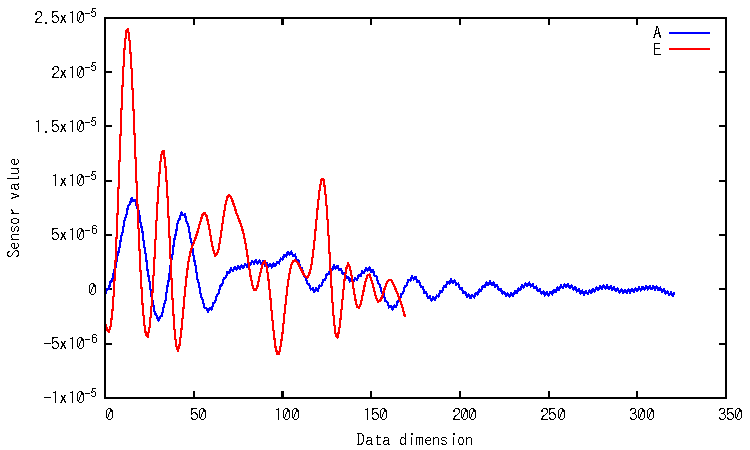
\includegraphics[bb=0 0 360 216, width=6cm]{Graphs/comp.pdf}
    \caption{被験者Aと被験者Eのデータ比較}
    \label{compare}
  \end{minipage}
\end{figure}


次に,登録及び認証処理にかかる時間を計測するための実験を行った.
